\documentclass[aps,prd,twocolumn,superscriptaddress,nofootinbib]{revtex4-2}
\usepackage{amsmath,amssymb,bm}
\usepackage{graphicx}
\usepackage{booktabs}
\usepackage{multirow}
\usepackage{siunitx}
\usepackage{url}
\usepackage{xcolor}
\sisetup{detect-all,scientific-notation=true,per-mode=symbol}
\newcommand{\MsunN}{M_{\odot}^{\rm N}}
\newcommand{\eps}{\varepsilon}
\newcommand{\mub}{\mu_{\rm B}}
\newcommand{\nb}{n_{\rm B}}
\newcommand{\cs}{c_{\rm s}}
\newcommand{\dd}{\mathrm{d}}
\newcommand{\Rstar}{R_\star}
\begin{document}

\title{Quadrupolar $f$- and $p_1$-mode frequencies of joined neutron-star equations of state in the relativistic Cowling approximation}

\author{[Author name(s) to be supplied]}
\date{\today}

\begin{abstract}
We calculate the quadrupolar polar-fluid fundamental mode and first pressure overtone of 234 crust--core joined neutron-star equations of state (EOSs). The cohort is drawn from a 390-member matching matrix containing 13 crust tables, three high-density core families, and six matching prescriptions; the 156 cases independently classified as retaining source-core acausality are excluded. Before stellar integration, the tabulated cold barotropes are represented by a thermodynamically consistent, causal piecewise-cubic $P(\mub)$ realization constructed from a monotone $q(\mub)=\nb/\mub$. The original tables are retained unchanged alongside these derived tables. For each EOS we solve the TOV equations at a fixed gravitational mass $M=1.3300106263\,\MsunN$ and locate the $\ell=2$ fluid roots by two-sided matching in the relativistic Cowling approximation. Eigenfunction node counts, rather than frequency ordering alone, identify the $f$ and $p_1$ modes. All 234 cases pass the node-identity and matching checks. Across the three core families, the median frequencies are respectively $(f,p_1)=(2.505,7.008)$ kHz for BBB\_BHF2, $(2.370,6.718)$ kHz for RG\_SLY4, and $(1.920,6.009)$ kHz for GM\_GM1. Tightening the ODE tolerances and step cap changes the frequencies of three representative models by at most $1.71\times10^{-6}$ Hz between the loose and tight runs. These small integration differences quantify numerical convergence within the adopted model; they do not quantify the systematic error of the Cowling approximation or the uncertainty associated with the barotropic, beta-equilibrated perturbation closure.
\end{abstract}

\maketitle

\section{Introduction}

Fluid oscillations of neutron stars provide a connection between the stellar bulk structure and the high-density equation of state. The fundamental fluid mode is predominantly restored by the star's global pressure and gravitational stratification, whereas pressure overtones are acoustic in character. Their frequencies therefore respond differently to the density dependence of the EOS. A mode label must, however, be tied to the eigenfunction: in a smooth barotropic problem the $f$ mode is nodeless, while the first pressure overtone has one radial node in the relevant fluid displacement functions \cite{Kokkotas1996,Finn1988}.

The fully relativistic nonradial problem couples fluid perturbations to metric perturbations and, for radiative modes, to an exterior gravitational-wave solution. The relativistic Cowling approximation fixes the background metric and neglects its Eulerian perturbation. It is consequently appropriate for a controlled calculation of fluid-mode frequencies, but it does not produce gravitational-wave damping times or spacetime $w$ modes. Comparisons with full general relativity show that the accuracy is mode- and compactness-dependent; differences of order ten to several tens of percent can occur, particularly for the $f$ mode in less compact configurations \cite{YoshidaKojima1997,Kokkotas1996}. A recent analysis also emphasizes that the response of matter during an oscillation need not coincide with the equilibrium beta-equilibrated response used to construct a cold barotropic EOS \cite{Montefusco2025}.

Here we apply the relativistic Cowling fluid equations supplied in the \texttt{Neutron\_Star\_Oscillations\_Seminar} package to a large set of joined CompOSE barotropes. We focus on the reproducible numerical spectrum of the stated model, not on a full-GR prediction. A necessary part of the calculation is to distinguish three logically separate questions: whether the original crust--core join passes its source-level gates, whether the EOS interpolant is a thermodynamically admissible function between its tabulated knots, and whether an eigenfrequency root has the node structure of the requested mode. The analysis preserves these distinctions.

\section{EOS cohort and thermodynamic representation}

\subsection{Joined-table cohort}

The starting matching matrix contains
\begin{equation}
N_{\rm matrix}=13\times 5\times 6=390
\end{equation}
candidate crust--core tables. An independent source audit classified 234 as passing the join-level consistency gates and 156 as retaining source-core acausality. The latter set comprises 78 APR\_APR and 78 RG\_KDE0v1 cases; it is not included in the oscillation calculation. No clipping, causal continuation, or post hoc promotion of these source failures is performed here.

The passing set consists of 13 crust tables joined to three core families, BBB\_BHF2, RG\_SLY4, and GM\_GM1, using six matching prescriptions labelled \texttt{css}, \texttt{cubic\_F}, \texttt{cubic\_P}, \texttt{maxwell}, \texttt{quintic\_F}, and \texttt{quintic\_P}. Thus each core family contributes 78 EOSs. The labels are inherited from the matching matrix. In particular, the suffix \texttt{maxwell} denotes the corresponding legacy matching prescription in this matrix; it must not be read as an instruction to insert a sharp first-order phase boundary into the oscillation equations. The present stellar backgrounds are treated as smooth one-dimensional barotropes. No material-interface transfer condition or interface $g$-mode is included.

\subsection{Cold thermodynamic identity}

The source CompOSE tables provide the cold beta-equilibrated barotrope on a discrete grid. In the conventions used by the normalizer, the thermodynamic columns give
\begin{equation}
P=\nb Q_1,\qquad
\mub=m_n(1+Q_3),\qquad
\eps=\nb m_n(1+Q_7),
\label{eq:compose}
\end{equation}
where $m_n$ is the neutron rest energy in the source-table convention. The first-law identity
\begin{equation}
\eps+P=\mub\nb
\label{eq:firstlaw}
\end{equation}
is checked at every source knot. For the 234 admitted tables the maximum relative residual of this identity is below $2\times10^{-12}$.

A direct use of the original pressure knots with the package's native cubic-Hermite $P(\mub)$ interpolant did not pass the package's cell-by-cell convexity and causality audit. This is an interpolation-admissibility issue and is kept separate from the earlier source-level acausality classification. To construct a causal interpolant without materially altering the tabulated density branch, we define
\begin{equation}
q(\mub)\equiv\frac{\nb}{\mub}.
\end{equation}
The nodal $q$ values are subjected to a weighted isotonic regression, giving a positive nondecreasing sequence. In each chemical-potential cell we take $q(\mub)$ to be linear and set
\begin{align}
\nb(\mub)&=\mub q(\mub),\\
P(\mub)&=P(\mu_{B,0})+\int_{\mu_{B,0}}^{\mub}
                 \tilde{\mub}\,q(\tilde{\mub})\,\dd\tilde{\mub},\\
\eps(\mub)&=\mub\nb(\mub)-P(\mub).
\label{eq:projection}
\end{align}
The integration constant is anchored to the original pressure at the first tabulated knot. Since $q$ is linear in a cell, $\nb$ is quadratic and $P$ is exactly cubic there. The resulting $P(\mub)$ is therefore represented exactly by a cubic-Hermite segment whose endpoint derivatives are the projected nodal densities.

The construction also makes the stability and causality conditions transparent:
\begin{equation}
\frac{\dd P}{\dd\mub}=\nb,\qquad
\frac{\dd\eps}{\dd\mub}=\mub\frac{\dd\nb}{\dd\mub},\qquad
\cs^2\equiv\frac{\dd P}{\dd\eps}
=\frac{q}{q+\mub q'}.
\label{eq:causality}
\end{equation}
For $q>0$ and $q'\geq0$, one has $0<\cs^2\leq1$. The projected density knots differ from the original density knots by at most $3.18\times10^{-16}$ in relative terms, i.e. at roundoff level. The pressure reconstructed from the first-law integral differs from the original pressure sequence by at most $1.2931\times10^{-3}P_{\max}$; the median of this maximum-per-table measure is $5.0781\times10^{-4}P_{\max}$. The maximum change in energy density, measured relative to $\mub\nb$, is $8.3590\times10^{-4}$. All 234 projected EOS tables pass every native interpolation cell in the package audit. Both source-normalized and projected tables are retained in the data release, so the projection is explicit and reversible at the file level.

\section{Relativistic Cowling problem}

\subsection{Background star}

We use the static, spherically symmetric metric
\begin{equation}
\dd s^2=-e^{2\nu(r)}c^2\dd t^2+e^{2\lambda(r)}\dd r^2
       +r^2\dd\Omega^2,
\end{equation}
with signature $(-,+,+,+)$ and
\begin{equation}
e^{-2\lambda}=1-\frac{2Gm(r)}{rc^2}.
\end{equation}
The TOV equations are
\begin{align}
\frac{\dd m}{\dd r}&=4\pi r^2\frac{\eps}{c^2},\\
\frac{\dd P}{\dd r}&=-(\eps+P)\frac{\dd\nu}{\dd r},\\
\frac{\dd\nu}{\dd r}
&=\frac{G\left[m+4\pi r^3P/c^2\right]}
{c^2r^2\left[1-2Gm/(rc^2)\right]}.
\end{align}
The lapse is normalized by the Schwarzschild exterior value at the adopted surface cutoff. The target gravitational mass is
\begin{equation}
M=2.644606257493485\times10^{30}\ {\rm kg}
 =1.3300106263\,\MsunN,
\end{equation}
where $\MsunN=(GM)_\odot^{\rm N}/G$ uses the IAU nominal solar mass parameter $(GM)_\odot^{\rm N}=1.3271244\times10^{20}\ {\rm m^3\,s^{-2}}$ and $G=6.67430\times10^{-11}\ {\rm m^3\,kg^{-1}\,s^{-2}}$. Each EOS is assigned its own central-pressure bracket on the low-pressure, increasing-mass branch; the mass is not obtained by applying one common central pressure to all EOSs.

The integration ends at the lowest positive pressure tabulated in the EOS, not at $P=0$. We therefore report radii and eigenfrequencies for a finite-pressure cutoff model. The cutoff pressure is reached exactly by the pressure-coordinate integration. The difference between a finite-cutoff surface and an exact vacuum surface is a model systematic not included in the ODE convergence table.

\subsection{Polar fluid perturbations}

We adopt harmonic time dependence $e^{i\omega t}$ and a polar displacement
\begin{equation}
\xi^r=e^{-\lambda}\frac{W(r)}{r^2}Y_{\ell m},\qquad
\xi^a=-\frac{V(r)}{r^2}D^aY_{\ell m}.
\end{equation}
With this convention $[W]=L^3$ and $[V]=L^2$. In the relativistic Cowling approximation the metric perturbation is set to zero. For $\ell=2$, the two first-order equations used in the package are
\begin{align}
Q&=\left(\frac{\omega r}{c}\right)^2e^{\lambda-2\nu}V
       +\nu'W,\label{eq:Q}\\
\frac{\dd W}{\dd r}&=\frac{Q}{\chi}-6e^\lambda V,\label{eq:W}\\
\frac{\dd V}{\dd r}&=2\nu'V-\frac{e^\lambda}{r^2}W,\label{eq:V}
\end{align}
where $\chi=\dd P/\dd\eps$ is the barotropic compressibility of the projected EOS. The regular central solution satisfies
\begin{equation}
W=A r^3+O(r^5),\qquad V=-\frac{A}{2}r^2+O(r^4).
\end{equation}
We use the package's second-order central expansion at $r_0=10$ m.

The Cowling surface condition is expressed in terms of the Lagrangian pressure perturbation,
\begin{equation}
\Delta P=-\frac{(\eps+P)e^{-\lambda}}{r^2}Q.
\end{equation}
Because the model ends at a positive cutoff pressure, the package's normalized surface residual is retained as a diagnostic rather than interpreted as an exact vacuum-boundary condition. Frequencies are located by matching independent inward and outward solutions at a fixed EOS-cell index. The normalized matching determinant is bisected in frequency.

\subsection{Mode identity}

A root is not labelled by frequency order alone. We count radial zeros of both $W$ and $V$ in the interior solution, using the package's relative zero threshold. A valid quadrupolar $f$ mode must have $(N_W,N_V)=(0,0)$ and a valid $p_1$ mode must have $(N_W,N_V)=(1,1)$. The corresponding outer branch is separately checked to be nodeless. This criterion is applied to all final models. An initial batch exposed 72 GM\_GM1 roots with three interior nodes; these were treated as higher-overtone candidates and not retained as $p_1$. The first one-node pressure root was found by a wider residual scan and the 72 cases were recomputed. The final 234-row set contains 234 nodeless $f$ roots and 234 one-node $p_1$ roots.

\section{Results}

\subsection{Core-family dependence}

Table~\ref{tab:families} summarizes the median and full range of the calculated frequencies and radii in each core family. Each group contains 78 EOSs and spans all 13 crust tables and six matching prescriptions. The $f$ and $p_1$ frequencies differ substantially between the core families at fixed gravitational mass. The spread within a family is smaller than the separation of the family medians for these three representative high-density core sets.

\begin{table*}[t]
\caption{Quadrupolar relativistic-Cowling frequencies and radii at $M=1.3300106263\,\MsunN$. Entries are the median followed by the full range across the 78 EOSs in each core family.}
\label{tab:families}
\begin{ruledtabular}
\begin{tabular}{lccc}
Core family & $f$ mode [kHz] & $p_1$ mode [kHz] & $\Rstar$ [km]\\
\midrule
BBB\_BHF2 & $2.5051\ [2.4883,\,2.5136]$ & $7.0083\ [6.6076,\,7.1823]$ & $11.2684\ [11.2653,\,11.2738]$\\
RG\_SLY4  & $2.3698\ [2.3574,\,2.3803]$ & $6.7177\ [6.3471,\,6.8906]$ & $11.7706\ [11.7670,\,11.7745]$\\
GM\_GM1   & $1.9202\ [1.8893,\,1.9401]$ & $6.0090\ [5.6866,\,6.0773]$ & $13.8079\ [13.7980,\,13.8215]$\\
\end{tabular}
\end{ruledtabular}
\end{table*}

The larger radii in the GM\_GM1 subset accompany its lower $f$- and $p_1$-mode frequencies in this fixed-mass comparison. This statement is descriptive for the selected table cohort; it is not a universal relation and should not be extrapolated to unrelated EOS families.

\begin{figure}[t]
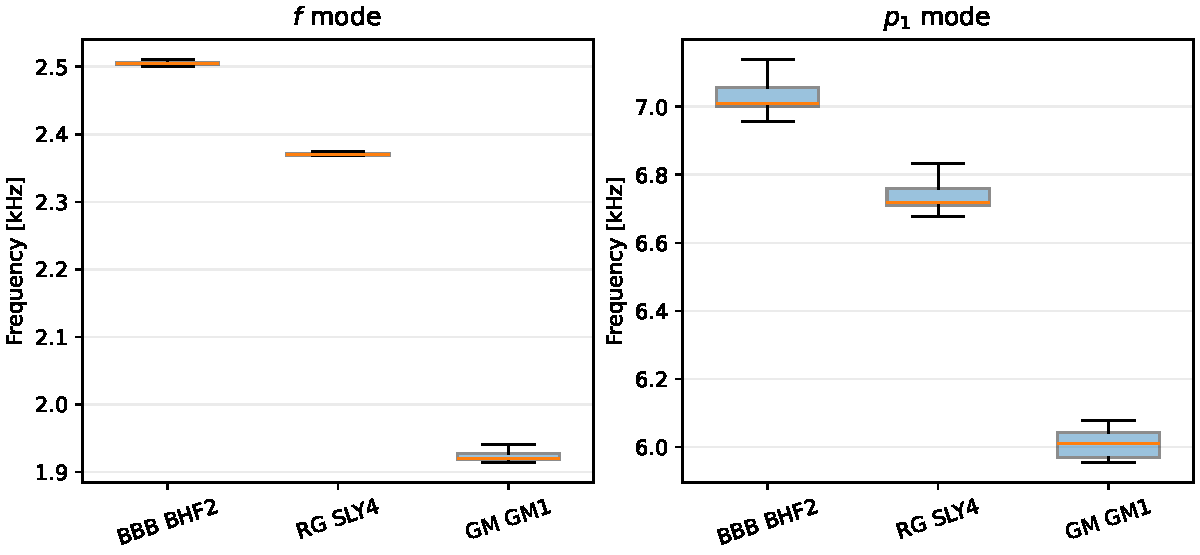
\includegraphics[width=\columnwidth]{fig_mode_frequencies.pdf}
\caption{Distribution of the quadrupolar $f$- and $p_1$-mode frequencies across the 78 EOSs in each core family. The spread includes the 13 crust choices and six matching prescriptions. Frequencies are calculated in the relativistic Cowling approximation.}
\label{fig:frequencies}
\end{figure}

\subsection{Numerical validation}

The maximum absolute normalized matching residual over the 234 EOSs is $4.56\times10^{-8}$ for the $f$ mode and $3.09\times10^{-10}$ for the $p_1$ mode. The maximum relative mass residual against the target mass is $9.92\times10^{-13}$. The largest inward--outward matching-radius mismatch is $9.10\times10^{-12}$ m and the largest relative matching-mass mismatch is $6.39\times10^{-16}$. The maximum absolute surface residual is $2.78\times10^{-17}$ for $p_1$; the surface pressure is reached with zero relative cutoff error at the stored precision. Every final mode satisfies the required node identity.

We also repeated three representative EOSs, one per core family, with progressively tighter ODE tolerances and smaller maximum step caps. The central pressure was held fixed in this convergence experiment, so the mass changes shown in the calculation archive reflect integration convergence rather than a new mass-target solve. Table~\ref{tab:convergence} reports the largest absolute difference between the loose and tight frequency results, as well as between the nominal and tight results.

\begin{table}[b]
\caption{Frequency convergence for three representative EOSs at fixed central pressure. The reported differences are absolute loose--tight and nominal--tight changes.}
\label{tab:convergence}
\begin{ruledtabular}
\begin{tabular}{lcc}
Core & $|f_{\rm loose}-f_{\rm tight}|$ [Hz] & $|p_{1,\rm loose}-p_{1,\rm tight}|$ [Hz]\\
\midrule
BBB\_BHF2 & $9.35\times10^{-8}$ & $1.71\times10^{-6}$\\
RG\_SLY4  & $6.64\times10^{-8}$ & $1.28\times10^{-7}$\\
GM\_GM1   & $1.80\times10^{-8}$ & $3.67\times10^{-7}$\\
\end{tabular}
\end{ruledtabular}
\end{table}

The maximum nominal--tight differences are $1.11\times10^{-8}$ Hz for $f$ and $4.98\times10^{-8}$ Hz for $p_1$. These numbers demonstrate convergence of the numerical integration and root-finding procedures for the representative cases. They are not rigorous global error bounds for all 234 EOSs and do not include interpolation systematics, finite surface-cutoff effects, uncertainty in the source EOS, or the error of the Cowling approximation.

\section{Discussion and limitations}

The results provide a systematic, node-identified spectrum for a large set of smooth crust--core joined cold barotropes under one declared relativistic fluid-oscillation model. They should not be interpreted as full general-relativistic mode frequencies. Neglecting metric perturbations changes the fluid-mode spectrum, and published comparisons show that the error depends on mode type and stellar compactness \cite{YoshidaKojima1997,Kokkotas1996}. The integration convergence measured here is many orders of magnitude tighter than those approximation-level differences; quoting many digits in the frequency table is useful for internal numerical comparisons, not a claim of comparable physical accuracy.

A second limitation is the perturbative thermodynamic closure. The equilibrium EOSs are cold beta-equilibrated barotropes, and the perturbation equations use the same equilibrium derivative $\chi=\dd P/\dd\eps$. Weak reactions may be too slow to maintain beta equilibrium during an oscillation, in which case the relevant adiabatic response is closer to a frozen-composition derivative. The difference between frozen and beta-equilibrated $f$ and $p$ modes has been studied explicitly for cold neutron-star matter \cite{Montefusco2025}. The present results do not implement that frozen-composition closure and should be treated as the beta-equilibrated barotropic Cowling spectrum.

The calculation also assumes a perfect fluid and spherical, nonrotating background. Elastic crust shear, superfluid counter-motion, magnetic stresses, rotational mode splitting, and sharp material-interface transfer conditions are absent. In particular, first-order phase transitions can introduce discontinuity-driven modes and require explicit interface conditions; such modes are not represented by the smooth one-dimensional tables used here \cite{RaneaSandoval2018}. The finite positive surface-pressure cutoff is another controlled numerical approximation and must be kept in mind when comparing the frequencies with calculations that integrate to a zero-pressure surface.

The thermodynamic reconstruction is a separate modeling step. It preserves the nodal density sequence to roundoff while reconstructing pressure and energy density from the first law so that the package's native cubic-Hermite interpolant is stable and causal cell by cell. The raw normalized EOS tables and the derived projected tables are both distributed. Consequently, downstream users can compare spectra based on the projected representation with alternative thermodynamically consistent interpolants without confusing the projection with a change in the original nuclear-model labels.

\section{Conclusions}

We have calculated the quadrupolar polar-fluid $f$ and first pressure $p_1$ mode frequencies for 234 source-audited crust--core joined EOSs at a common mass of $1.3300106263\,\MsunN$. The computation uses the relativistic Cowling approximation, a cold beta-equilibrated barotropic closure, a finite positive surface-pressure cutoff, and two-sided matching in the package's native EOS cells. A monotone-$q(\mub)$ thermodynamic reconstruction was required for all 234 joined tables to pass the package's cellwise interpolation audit. Each final root passes the expected eigenfunction node identity, matching, mass, and surface diagnostics. The three core families show clearly separated median frequencies in this cohort. The numerical convergence tests are substantially tighter than the known model systematics of the Cowling and barotropic approximations, which remain the dominant interpretive limitations.

\begin{acknowledgments}
The numerical calculations used the Fortran TOV and relativistic-Cowling implementation distributed in the supplied \texttt{Neutron\_Star\_Oscillations\_Seminar} package. The release archive records the input package checksum, source EOS provenance, projected EOS hashes, solver settings, run manifests, and validation summaries.
\end{acknowledgments}

\bibliographystyle{apsrev4-2}
\bibliography{references}
\end{document}
